%************************************************
\chapter{Introduction}\label{ch:introduction}
%************************************************

The Standard Model of particle physics, which describes the fundamental constituents of matter and their interactions, represents an unambiguous triumph of the scientific method. Its predictions have been verified to extraordinary precision. The last missing piece of the standard model, the Higgs boson, was discovered in 2012, fifty years after it was predicted. This resulted in a Nobel prize for Francois Englert and Peter Higgs, and in much jubilation among the particle physics community. However, 

\begin{figure}
  \centering
  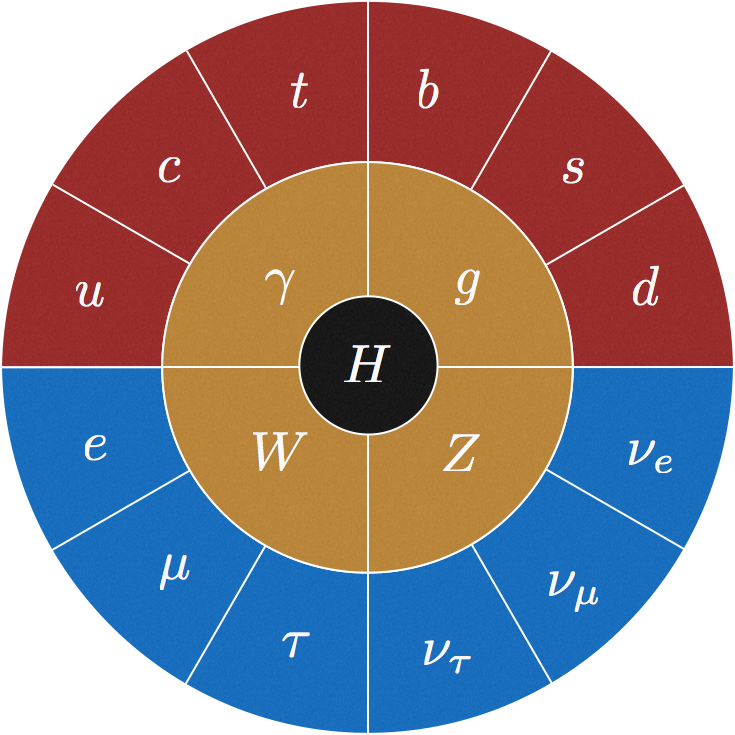
\includegraphics[width=0.35\textwidth]{gfx/SM-wheel.png}
  \caption{Graphical representation of the particle content of the standard model.}
\end{figure}



